\documentclass{beamer}
\usepackage{multirow}

\usetheme{Padova}

\title{\textbf{ADeQA: una \textit{progressive web app} per il controllo qualità industriale}}
\subtitle{Dipartimento di Matematica "Tullio Levi Civita" \\ Corso di Laurea in Informatica}
\author{Matteo Cusin}
\date{13 Dicembre, 2023}


\begin{document}
\setcounter{framenumber}{-2}
	\maketitle
	\begin{frame}{Indice}
		\tableofcontents 
	\end{frame}

	\setcounter{framenumber}{0}

	\section{Contesto di svolgimento delle attività} 
	\begin{frame}{Contesto di svolgimento delle attività}

		{\LARGE \textbf{L'azienda}} \hspace*{0.7\textwidth} 
\includegraphics[width=3cm]{images/logo_azienda.png}
		\vspace{1cm}
		\hspace{-1cm}
	
		% \begin{tabular}{cc}
		% 	\hline
		% 	\begin{tabular}{c}
		% 		\parbox{0.7\linewidth}{%  change the parbox width as appropiate
		% 		\begin{itemize}
		% 			\setlength\itemsep{1em}
		% 			\item \textit{Software house} nata nel 2012, sede legale a Monselice(PD);
		% 			\item Specializzata nella consulenza e nello sviluppo di soluzioni \textit{business to business}
		% 				\begin{itemize}
		% 					\item \textit{Warehouse management system};
		% 					\item \textit{Manifacturing execution system} ;
		% 					\item \textit{Digital management assets}.
		% 				\end{itemize}
		% 		\end{itemize}
		% 		}
		% 	\end{tabular}
		% 	& \vspace*{-1cm}
		% 	\begin{tabular}{c}
		% 		\hline
		% 		
\includegraphics[width=3cm]{images/logo_azienda.png}
		% 	  \end{tabular}
   		% \end{tabular}
			\begin{tabular}{cc}
				\hspace*{-1cm}
				\begin{tabular}{c}
				  \parbox{0.65\linewidth}{%
					\begin{itemize}
					  \setlength\itemsep{1em}
					  \item \textit{Software house} nata nel 2012, sede legale a Monselice(PD);
					  \item Specializzata nella consulenza e nello sviluppo di soluzioni \textit{business to business}
							\begin{itemize}
							  \item \textit{Warehouse management system};
							  \item \textit{Manifacturing execution system} ;
							  \item \textit{Digital management assets}.
							\end{itemize}
					\end{itemize}
				  }
				\end{tabular}%
			  & \hspace*{-2cm}
			  \begin{tabular}{c}
				\parbox{0.35\linewidth}{%
				  \begin{itemize}
					\setlength\itemsep{1em}
					\item[] 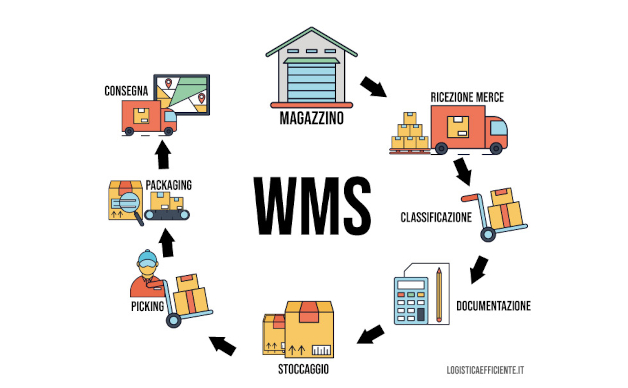
\includegraphics[width=6cm]{images/wms.jpg}
				  \end{itemize}
				}
			  \end{tabular}
			\end{tabular}

	\end{frame}

	\section{Motivazioni alla base del tirocinio}
	\begin{frame}{Motivazioni alla base del tirocinio}
		% \begin{block}{Normal block}
		% 	Fusce luctus venenatis felis quis semper
		% \end{block}

		% \begin{alertblock}{Alert block}
		% 	$$ E = (x_1 \vee \neg x_2 \vee \neg x_3) \wedge (x_1 \vee x_2 \vee x_4) $$
		% \end{alertblock}

		% \begin{exampleblock}{Example block}
		% 	Proin tincidunt, neque at tincidunt mollis
		% \end{exampleblock}
	\end{frame}

	\section{Elementi caratterizzanti del progetto}
	\begin{frame}{Elementi caratterizzanti del progetto}
		Ciao
	\end{frame} 

	\section{Retrospettiva delle attività} 
	\begin{frame}{Retrospettiva delle attività}
		Ciao
	\end{frame}

\end{document}
